\documentclass[a4paper]{article}
\usepackage[utf8]{inputenc}
\usepackage[russian,english]{babel}
\usepackage[T2A]{fontenc}
\usepackage[left=10mm, top=20mm, right=18mm, bottom=15mm, footskip=10mm]{geometry}
\usepackage{indentfirst}
\usepackage{amsmath,amssymb}
\usepackage[italicdiff]{physics}
\usepackage{graphicx}
\graphicspath{{images/}}
\DeclareGraphicsExtensions{.pdf,.png,.jpg}
\usepackage{wrapfig}

\usepackage{caption}
\captionsetup[figure]{name=Рисунок}
\captionsetup[table]{name=Таблица}
  
\title{\underline{Отчет о выполненой лабораторной работе 1.4.5}}
\author{Воронин Денис, Б04-403}

\begin{document}

\maketitle

\begin{center}
\textbf{\Large Изучение колебаний струны}
\end{center}

\section{Аннотация}
\underline{Цель работы}: 
Изучить поперечные стоячие волн на тонкой натянутой струне; измерить собственные частоты колебаний струны и проверить условие образования стоячих волн; измерить скорость распространения поперечных волн на струне и исследовать её зависимость от натяжения струны.

\underline{Оборудование}: 
В работе используются: закрепленная на станине стальная струна, набор грузов, электромагнитные датчики, звуковой генератор, двухканальный осциллограф, частотомер.

\section{Теоретические сведения}\par

Струной в акустике называют однородную тонкую гибкую упругую нить. Примерами могут служить сильно натянутый шнур или трос, струны гитары, скрипки и других музыкальных инструментов. В данной работе изучаются поперечные колебания стальной гитарной струны, натянутой горизонтально и закрепленной между двумя неподвижными зажимами. Основное свойство струны — гибкость — обусловлено тем, что её поперечные размеры малы по сравнению с длиной. Это означает, что напряжение в струне может быть направлено только вдоль неё, и позволяет не учитывать изгибные напряжения, которые могли бы возникать при поперечных деформациях (то есть при изгибе струны).
В натянутой струне возникает поперечная упругость, т.е. способность сопротивляться всякому изменению формы, происходящему без изменения объема. При вертикальном смещении произвольного элемента струны, возникают силы, действующие на соседние элементы, и в результате вся струна приходит в движение в вертикальной плоскости, т.е. возбуждение «бежит» по струне. Передача возбуждения представляет собой поперечные бегущие волны, распространяющиеся с некоторой скоростью в обе стороны от места возбуждения. В ненатянутом состоянии струна не обладает свойством поперечной упругости, и поперечные волны на ней невозможны.

\underline{Уравнение волны на струне}:\par

Рассмотрим гибкую однородную струну, в которой создано натяжение $T$, и получим дифференциальное уравнение, описывающее её малые поперечные свободные колебания. Отметим, что, если струна расположена горизонтально в поле тяжести, величина $T$ должна быть достаточна для того, чтобы в состоянии равновесия струна не провисала, т.е. сила натяжения должна существенно превышать вес струны.

\underline{Волновое уравнение}:\par

\[\frac{d^2y}{dt^2} = u^2\frac{d^2y}{dx^2}\]
\[u = \sqrt{\frac{T}{\rho_{l}}}\]
\underline{Бегущие волны}:\par

Волновое уравнение представимо в виде суммы двух бегущих волн:
\[y(x,t) = y_{1}(x - ut) + y_{2}(x + ut)\]
Для гармонических волн будет:
\[y(x,t) = a cos(\omega t - kx) + b cos(\omega t + kx), u = \frac{\omega}{k} = \nu \lambda\]
Здесь длина волны $\lambda = \frac{2\pi}{k}, \text{частота } \nu = \frac{\omega}{2\pi} . \text{Величина } k = \frac{2\pi}{\lambda}$ называется волновым числом или пространственной частотой волны.

\underline{Собственные колебания струны. Стоячие волны}:\par

Свободные колебания струны с закрепленными концами
\[y(x,t) = 2a sin(kx) \cdot sin(\omega t)\]
Стоячие волны на струне с закреплёнными концами образуются, только если на длине струны укладывается целое число полуволн:
\[\lambda_{n} = \frac{2L}{n}, L - \text{длина закрепления}\]
Частота колебания струны будет:
\[\nu_{n} = \frac{u}{\lambda_{n}} = \frac{n}{2L}\sqrt{\frac{T}{\rho_{l}}},\text{где $\rho_{l}$ - погонная плотность, $T$ - сила натяжения, $L$ - длина струны, n - номер гармоники.}\]

\begin{figure}[t]
    \centering
    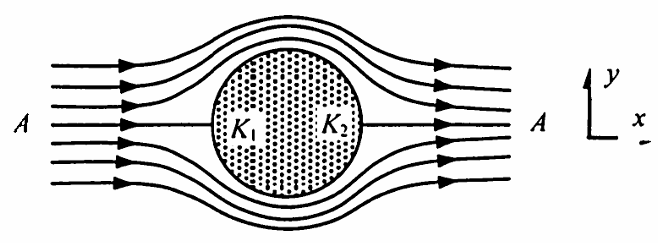
\includegraphics[width=0.6\textwidth]{pick1.png}
    \caption{Экспериментальная установка}
\end{figure}

\underline{Экспериментальная установка} \newline
\par
Стальная гитарная струна 1 закрепляется в горизонтальном положении между двумя стойками с зажимами 2 и 3, расположенными на массивной станине 4. Один конец струны закреплен в зажиме 2 неподвижно. К противоположному концу струны, перекинутому через блок, прикреплена платформа с грузами 5, создающими натяжение струны. Зажим 3 можно передвигать по станине, устанавливая требуемую длину струны. Возбуждение и регистрация колебаний струны осуществляются с помощью электромагнитных датчиков (вибраторов), расположенных на станине под струной. Электромагнитный датчик 6 подключен к звуковому генератору 7 и служит для возбуждения колебаний струны, частота которых измеряется с помощью частотомера 10 (в некоторых установках частотомер встроен в генератор). Колебания струны регистрируются с помощью электромагнитного датчика 8, сигнал с которого передается на вход осциллографа 9. Разъёмы, через которые датчики с помощью кабелей соединяются с генератором и осциллографом, расположены на корпусе станины.\par

Для регистрации колебаний струны в работе используется электронный осциллограф, соединённый с электромагнитным датчиком 8. Он позволяет регистрировать колебания в случаях, когда это невозможно сделать визуально. Также с помощью осциллографа можно измерять амплитуду возбуждения и форму сигнала, что даёт возможность установить, является ли режим возбуждения стоячих волн линейным, иными словами, имеет ли место прямая пропорциональность между силой возбуждения и амплитудой колебаний струны.
\newpage


\section{Данные}

На экспериментальной установке в зависимости от суммарной массы было сделано по 5 замеров для четных и 4 для нечетных гармоник для каждого из 5 опытов.
Используемые зависимости:
\[u = \sqrt{\frac{T}{\rho_{l}}}\]
\[\nu_{n} = u \cdot \frac{n}{2L} = \frac{n}{2L}\sqrt{\frac{T}{\rho_{l}}}\]


\begin{itemize}
    \item Длина струны постоянна и равна $L = 50 \text{ см} = 0,5 \text{ м}$ 
    \item Погонная плотность $\rho_{l} = 568,4 \text{ мг/м} $
\end{itemize}

\begin{table}[!h]
\begin{tabular}{|l|l|l|l|l|l|}
\hline
                    & 1     & 2     & 3   & 4     & 5     \\ \hline
    Общая масса, г & 1099,2 & 1590,7 & 2085,3 & 2579,9 & 3074,9 \\ \hline
\end{tabular}
\end{table}
Занесем полученные данные в таблицу:
\begin{table}[!h]
    \begin{tabular}{|c|ccc|ccc|ccc|ccc|ccc|}
    \hline
    Опыт                                                     & \multicolumn{3}{c|}{№1}                                                         & \multicolumn{3}{c|}{№2}                                                         & \multicolumn{3}{c|}{№3}                                                         & \multicolumn{3}{c|}{№4}                                                         & \multicolumn{3}{c|}{№5}                                                         \\ \hline
    \begin{tabular}[c]{@{}c@{}}Сила\\ натяжения\end{tabular} & \multicolumn{3}{c|}{10,78 Н}                                                  & \multicolumn{3}{c|}{15,6 Н}                                                    & \multicolumn{3}{c|}{20,5 Н}                                                    & \multicolumn{3}{c|}{25,3 Н}                                                    & \multicolumn{3}{c|}{30,2 Н}                                                   \\ \hline
                                                             & \multicolumn{1}{c|}{n}  & \multicolumn{1}{c|}{$\nu_{0}, Гц$} & $\nu_{real}, Гц$ & \multicolumn{1}{c|}{n}  & \multicolumn{1}{c|}{$\nu_{0}, Гц$} & $\nu_{real}, Гц$ & \multicolumn{1}{c|}{n}  & \multicolumn{1}{c|}{$\nu_{0}, Гц$} & $\nu_{real}, Гц$ & \multicolumn{1}{c|}{n}  & \multicolumn{1}{c|}{$\nu_{0}, Гц$} & $\nu_{real}, Гц$ & \multicolumn{1}{c|}{n}  & \multicolumn{1}{c|}{$\nu_{0}, Гц$} & $\nu_{real}, Гц$ \\ \hline
                                                             & \multicolumn{1}{c|}{1}  & \multicolumn{1}{c|}{137,8}         & 137              & \multicolumn{1}{c|}{1}  & \multicolumn{1}{c|}{165,2}         & 165,2            & \multicolumn{1}{c|}{1}  & \multicolumn{1}{c|}{189,7}         & 189              & \multicolumn{1}{c|}{1}  & \multicolumn{1}{c|}{210,9}         & 210,4              & \multicolumn{1}{c|}{1}  & \multicolumn{1}{c|}{230,37}         & 231,0            \\ \hline
                                                             & \multicolumn{1}{c|}{3}  & \multicolumn{1}{c|}{413,4}         & 412              & \multicolumn{1}{c|}{3}  & \multicolumn{1}{c|}{497,1}         & 498,5              & \multicolumn{1}{c|}{3}  & \multicolumn{1}{c|}{569,7}         & 570,6              & \multicolumn{1}{c|}{3}  & \multicolumn{1}{c|}{624,3}         & 634,6              & \multicolumn{1}{c|}{3}  & \multicolumn{1}{c|}{682,5}         & 693,0              \\ \hline
                                                             & \multicolumn{1}{c|}{5}  & \multicolumn{1}{c|}{689}           & 695              & \multicolumn{1}{c|}{5}  & \multicolumn{1}{c|}{829,0}         & 832,5              & \multicolumn{1}{c|}{5}  & \multicolumn{1}{c|}{949,5}         & 951,6              & \multicolumn{1}{c|}{5}  & \multicolumn{1}{c|}{1040,5}        & 1058,8             & \multicolumn{1}{c|}{5}  & \multicolumn{1}{c|}{1137,5}        & 1156,3             \\ \hline
                                                             & \multicolumn{1}{c|}{7}  & \multicolumn{1}{c|}{964,6}         & 974,8              & \multicolumn{1}{c|}{7}  & \multicolumn{1}{c|}{1160,7}        & 1168,2             & \multicolumn{1}{c|}{7}  & \multicolumn{1}{c|}{1329,3}        & 1334,7             & \multicolumn{1}{c|}{7}  & \multicolumn{1}{c|}{1456,7}        & 1484,5             & \multicolumn{1}{c|}{7}  & \multicolumn{1}{c|}{1592,5}        & 1621,6             \\ \hline
                                                             & \multicolumn{1}{c|}{9}  & \multicolumn{1}{c|}{1240,2}        & 1259,6            & \multicolumn{1}{c|}{9}  & \multicolumn{1}{c|}{1492,5}        & 1507,5             & \multicolumn{1}{c|}{9}  & \multicolumn{1}{c|}{1709,1}        & 1721,3             & \multicolumn{1}{c|}{9}  & \multicolumn{1}{c|}{1872,9}        & 1912,5             & \multicolumn{1}{c|}{9}  & \multicolumn{1}{c|}{2047,5}        & 2088,5             \\ \hline
                                                             & \multicolumn{1}{c|}{2}  & \multicolumn{1}{c|}{275,6}         & 276,5              & \multicolumn{1}{c|}{2}  & \multicolumn{1}{c|}{331,2}         & 332,2              & \multicolumn{1}{c|}{2}  & \multicolumn{1}{c|}{379,8}         & 379,2              & \multicolumn{1}{c|}{2}  & \multicolumn{1}{c|}{416,2}         & 422,4              & \multicolumn{1}{c|}{2}  & \multicolumn{1}{c|}{455}           & 462,0              \\ \hline
                                                             & \multicolumn{1}{c|}{4}  & \multicolumn{1}{c|}{551,2}         & 553,9               & \multicolumn{1}{c|}{4}  & \multicolumn{1}{c|}{663,0}         & 666,5              & \multicolumn{1}{c|}{4}  & \multicolumn{1}{c|}{759,6}         & 761,1              & \multicolumn{1}{c|}{4}  & \multicolumn{1}{c|}{832,4}         & 845,3              & \multicolumn{1}{c|}{4}  & \multicolumn{1}{c|}{910}           & 925,0              \\ \hline
                                                             & \multicolumn{1}{c|}{6}  & \multicolumn{1}{c|}{826,8}         & 834,0              & \multicolumn{1}{c|}{6}  & \multicolumn{1}{c|}{994,8}         & 1000,4              & \multicolumn{1}{c|}{6}  & \multicolumn{1}{c|}{1139,4}        & 1144,0             & \multicolumn{1}{c|}{6}  & \multicolumn{1}{c|}{1248,6}        & 1276,5             & \multicolumn{1}{c|}{6}  & \multicolumn{1}{c|}{1365}          & 1388,8             \\ \hline
                                                             & \multicolumn{1}{c|}{8}  & \multicolumn{1}{c|}{1102,4}        & 1117,4             & \multicolumn{1}{c|}{8}  & \multicolumn{1}{c|}{1326,0}        & 1338,9             & \multicolumn{1}{c|}{8}  & \multicolumn{1}{c|}{1519,2}        & 1527,7             & \multicolumn{1}{c|}{8}  & \multicolumn{1}{c|}{1664,8}        & 1698,9             & \multicolumn{1}{c|}{8}  & \multicolumn{1}{c|}{1820}          & 1854,7             \\ \hline
    
    \end{tabular}
    \end{table}


\section{Обработка результатов}

На основе данных эксперимента были построены графики $\nu_{real}(n), \nu_{0}(n)$,реальной частоты от n и расчетной частоты от n.
Для графика 
Получаем что при увеличении натяжения $T$ увеличивается и $u$ и при этом растет разница между рассчитываемыми и реальными значениями u. 

Погрешность образуется из случайной и систематической: погрешность при измерении длины  $\sigma_{L} = 0,0005$, пренебрежем погрешностями генератора частот и осцилографа
\[\text{Среднее значение:  } \overline{u} = \frac{1}{9}\sum\limits_{i=1}^{9} u_{i} \approx 137,3\]
\[\text{Среднеквадратическое отклонение:  } \sigma_{u} = \sqrt{\frac{1}{9}\sum\limits_{i=1}^{9} (u_{i} - \overline{u})^2} \approx 0,97\]
\[\text{Погрешность среднего значения(случайная):  } \sigma_{u}^{\text{случ}} = \frac{\sigma_{u}}{\sqrt{10}} \approx 0,3\]
\[\text{Систематическая погрешность:  }\sigma_{u}^{\text{сист}} = u\sqrt{\left( \frac{du}{dT}\right)^2 \sigma_{T}^2} = u \cdot \sigma_{L} \approx 0,069\]
\[\text{Полная погрешность:  }\sigma_{u}^{\text{полн}} = \sqrt{\sigma_{\text{сист}}^2 + \sigma_{\text{случ}}^2} \approx 0,3\]
Получаем $u = 137,3 \pm 0,3 (\varepsilon_{u} = 0,2\%)$ для натяжения T = 10,78 Н

Аналогично для погонной плотности $\rho_{l}$ получаем:
\[\text{Среднее значение:  } \overline{\rho} = \frac{1}{9}\sum\limits_{i=1}^{9} \rho_{i} \approx 567,9\]
\[\text{Среднеквадратическое отклонение:  } \sigma_{\rho} = \sqrt{\frac{1}{9}\sum\limits_{i=1}^{9} (\rho_{i} - \overline{\rho})^2} \approx 0,64\]
\[\text{Погрешность среднего значения(случайная):  } \sigma_{\rho}^{\text{случ}} = \frac{\sigma_{\rho}}{\sqrt{5}} \approx 0,36\]
\[\text{Систематическая погрешность:  }\sigma_{\rho}^{\text{сист}} = \rho\sqrt{\left( \frac{d\rho}{du}\right)^2 \sigma_{u}^2} = \rho \cdot 2\sigma_{u}\approx 2,3\]
\[\text{Полная погрешность:  }\sigma_{\rho}^{\text{полн}} = \sqrt{\sigma_{\text{сист}}^2 + \sigma_{\text{случ}}^2} \approx 2,3\]
Получаем $\rho_{l} = 570,5 \pm 2,3 \text{мг}/\text{м} (\varepsilon_{\rho} = 0,4\%)$\par

\newpage
\begin{figure}[t]
    \centering
    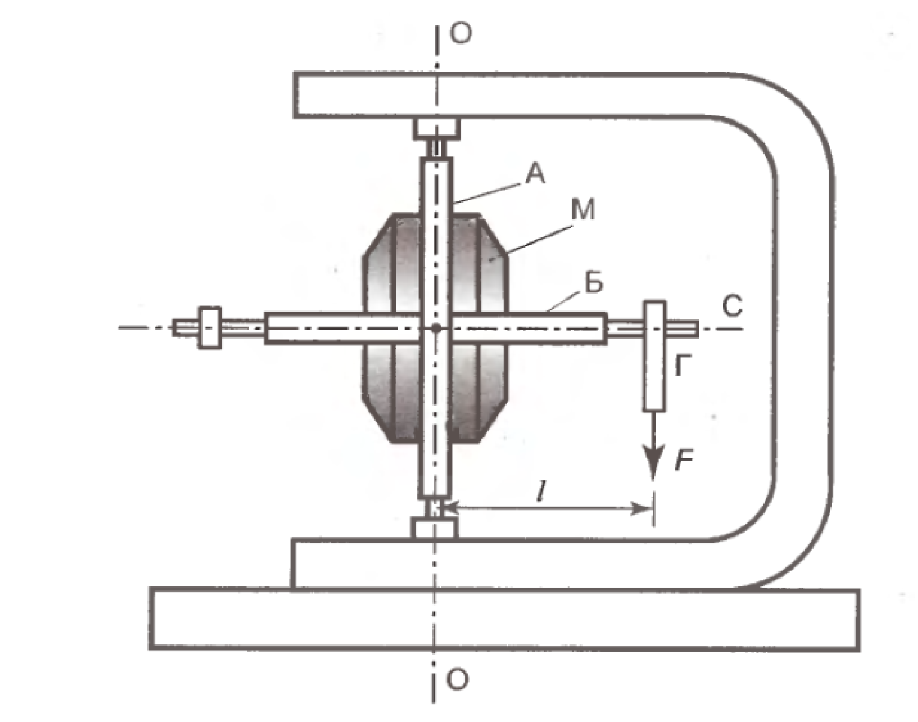
\includegraphics[width=0.8\textwidth]{pick2.png}
    \caption{Зависимость $\nu_{real}(n)$ реальной частоты от номера n гармоники с аппроксимирующими прямыми для 5 разных натяжений}
\end{figure}

\begin{figure}[t]
    \centering
    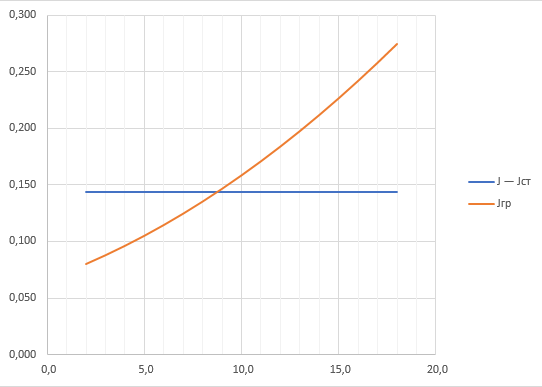
\includegraphics[width=0.7\textwidth]{pick3.png}
    \caption{Попадание мнк на прямую}
\end{figure}


\begin{figure}[t]
    \centering
    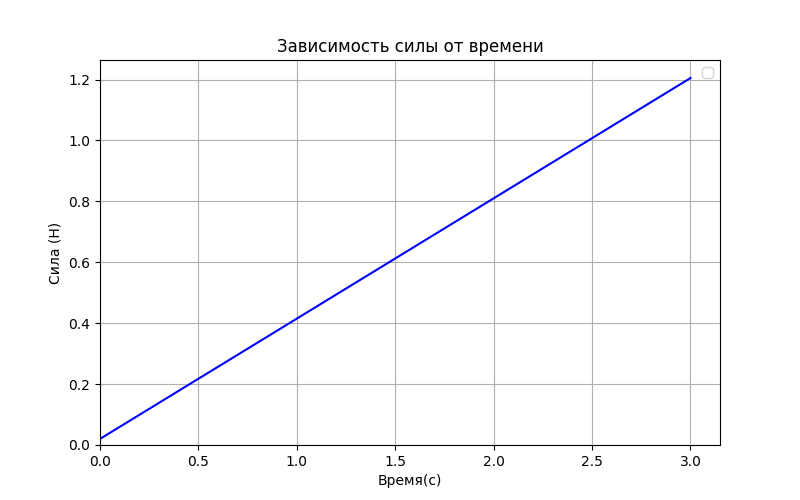
\includegraphics[width=0.8\textwidth]{pick4.png}
    \caption{Зависимость $u^2(T)$ и расчет погонной плотности $\rho_{l}$}
\end{figure}

\begin{figure}[t]
    \centering
    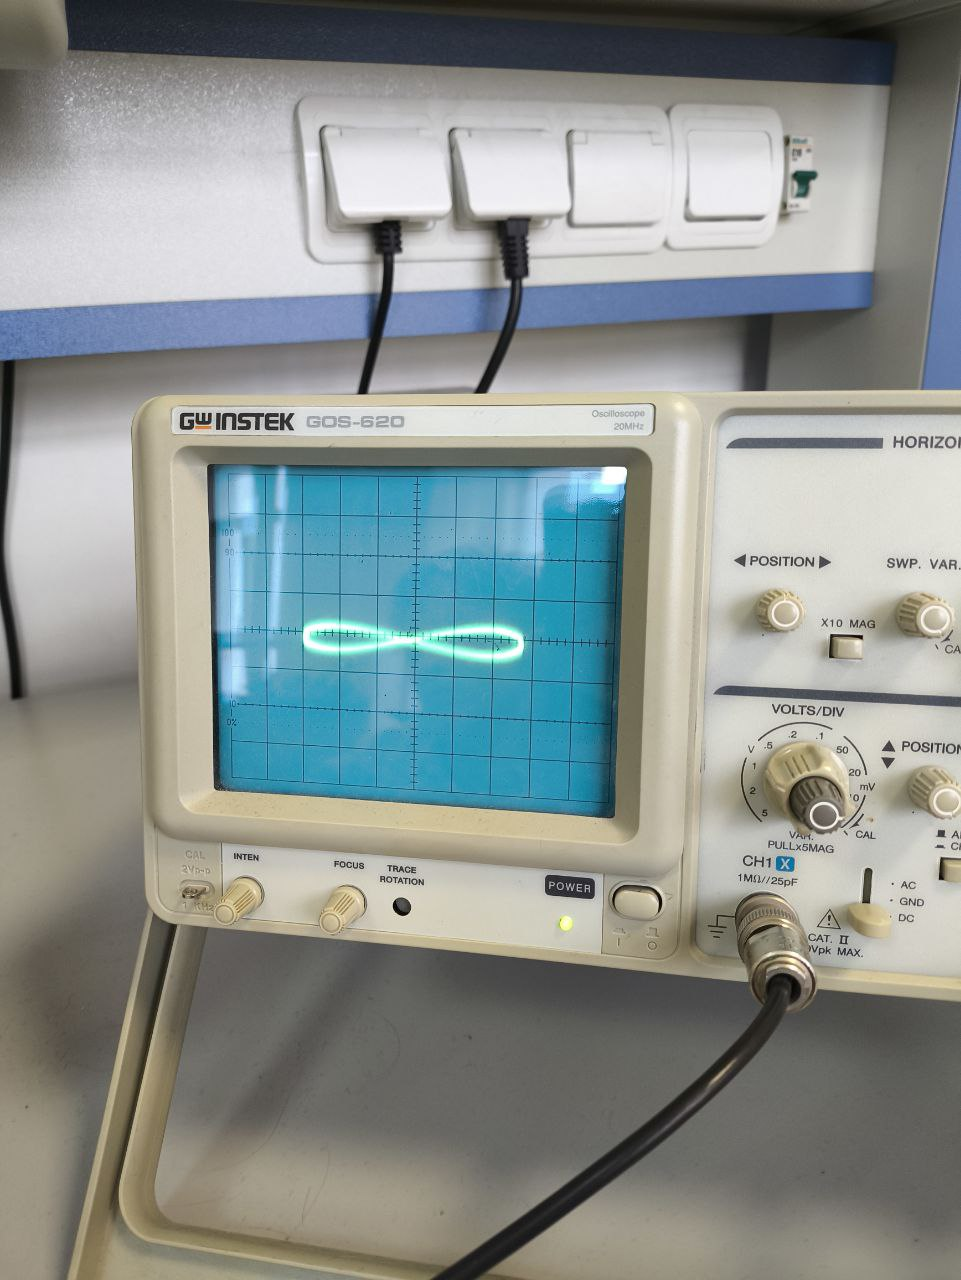
\includegraphics[width=0.5\textwidth]{pick5.jpg}
    \caption{Нахождение частоты с помощью фигур Лиссажу}
\end{figure}



\end{document}